For task 1, we focus on Principal Component Analysis (PCA), which is a dimensionality reduction technique used in statistical data analysis and machine learning. It simplifies complex datasets with high dimensions while attempting to preserve the essential patterns and relationships. PCA focuses on identifying the principal components that capture the most variance within a dataset. These components are orthogonal vectors representing the directions of maximum variance. PCA involves calculating the covariance matrix of the data and its eigendecomposition. The eigenvectors of the covariance matrix correspond to the principal components, and the eigenvalues indicate the amount of variance captured by each component. 

Given a dataset $\mathbf{X}$ with $m$ samples and $n$ features, PCA consists of the following steps:

\begin{enumerate}
  \item Standardize the dataset.
  \item Compute the covariance matrix $\Sigma = \frac{1}{m-1} \mathbf{X}^T \mathbf{X}$.
  \item Find the eigenvectors ($\mathbf{v}$) and eigenvalues ($\lambda$) of $\Sigma$.
  \item Sort eigenvectors by decreasing eigenvalues and form a feature vector $\mathbf{W}$.
  \item Project $\mathbf{X}$ onto the new subspace: $\mathbf{Y} = \mathbf{X} \mathbf{W}$.
\end{enumerate}
But, PCA also has its limitations. It is sensitive to the scale of the features, emphasizing the importance of standardization. Moreover, PCA assumes linear relationships and may not perform optimally with non-linear data. Also, determining the number of components to retain is crucial, often based on the explained variance.

We are implementing PCA on three different datasets using our custom Python script, 'PCA.py', designed to perform Singular Value Decomposition. This file handles preprocessing needs, including data normalization, and also offers customization for selecting the number of components based on the dataset's characteristics. It evaluates PCA performance through metrics like explained variance, complemented by visual tools for result interpretation. Compatible with recent Python versions and dependent on standard libraries, it integrates into different analytical workflows.

\begin{itemize}
    \item \textbf{Part 1:} \\
    Part 1 involves a two-dimensional dataset, \texttt{pca\_dataset.txt}. We implemented PCA with 2 components. The variance explained by each component is [0.99314266, 0.00685734], summing to an overall variance of approximately 1.0.
    \begin{figure}[H]
    \centering
    \begin{subfigure}[b]{0.45\textwidth}
        \centering
        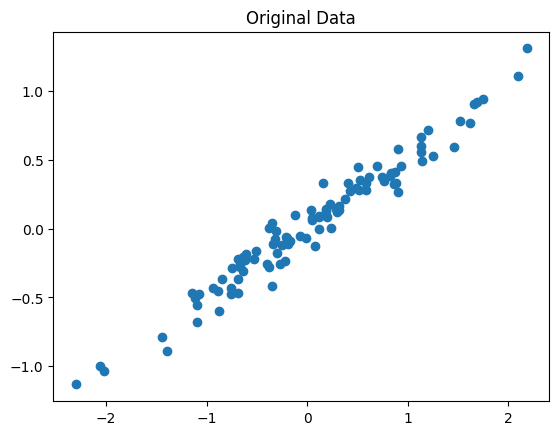
\includegraphics[width=\textwidth]{images/ex3task1-1-1.png}
        \caption{Dataset Plotted}
        \label{fig:Dataset Plotted}
    \end{subfigure}
    \begin{subfigure}[b]{0.45\textwidth}
        \centering
        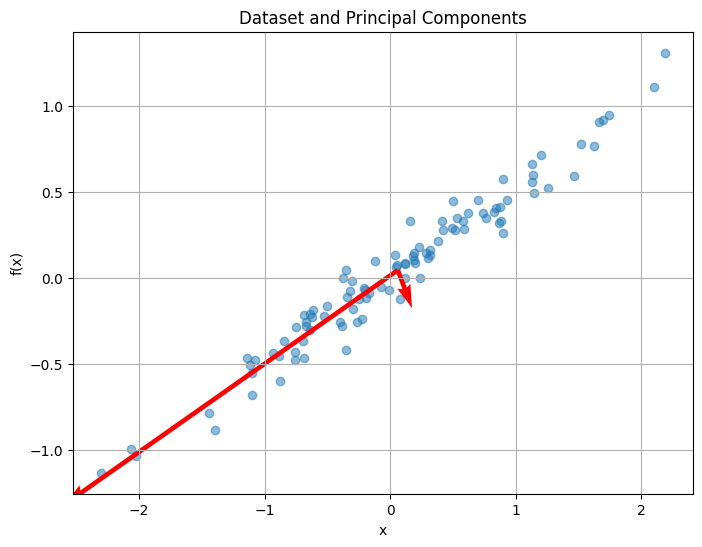
\includegraphics[width=\textwidth]{images/ex3task1-1-2.png}
        \caption{Dataset and Principal Components Plotted}
        \label{fig:Dataset and Principal Components Plotted}
    \end{subfigure}
    \caption{PCA on 2D Dataset}
    \label{fig:part1}
\end{figure}

What we learned from the results of PCA (see figure \ref{fig:part1}).
    \begin{itemize}
        \item This data appears linear and exhibits similar scale.
        \item There are a few data points that are far from the main cluster of data, particularly on the upper right side of the plot. These may be outliers that could potentially influence the PCA.
        \item  The longer red line points in the direction of the first principal component. This is the direction of greatest variance in the dataset. In PCA, this component would capture the most information about the data's structure. The shorter red line is the second principal component, it is orthogonal (at a right angle) to the first. It accounts for the next highest variance in the dataset and is uncorrelated with the first component. 
        \item The PCA seems to be centered around the mean (not necessarily at zero), suggesting that the data has been mean-centered before the PCA was performed.
    \end{itemize}
 

\item \textbf{Part 2:} \\
In Part 2, we analyze an image from the SciPy library. Due to a deprecation warning in SciPy v1.10.0 regarding \texttt{scipy.misc.face}, we have utilized \texttt{scipy.datasets.face} as an alternative. This function retrieves the classic 'face' image, which we use for PCA reconstruction.

\begin{figure}[H]
    \centering
    \begin{subfigure}[b]{0.5\textwidth}
        \centering
        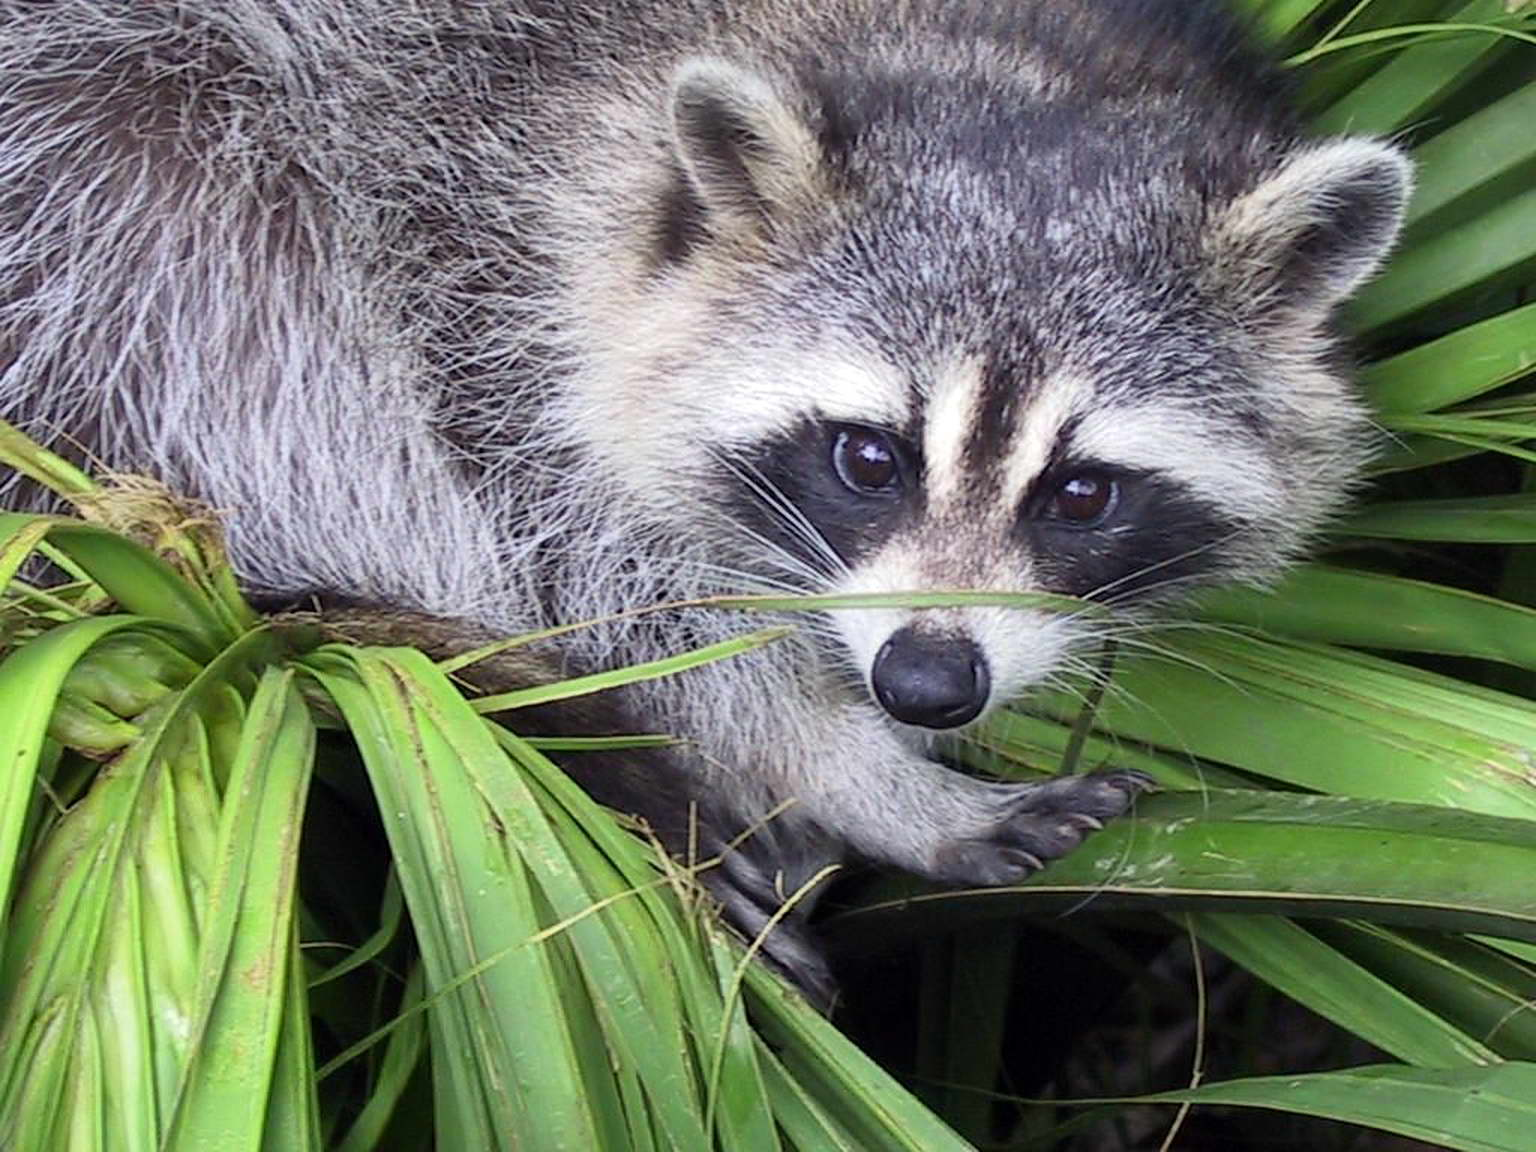
\includegraphics[width=\textwidth]{images/ex3task1-2-1.jpg}
        \caption{Original Image (Before Resizing)}
        \label{fig:original_image}
    \end{subfigure}
    \begin{subfigure}[b]{0.7\textwidth}
        \centering
        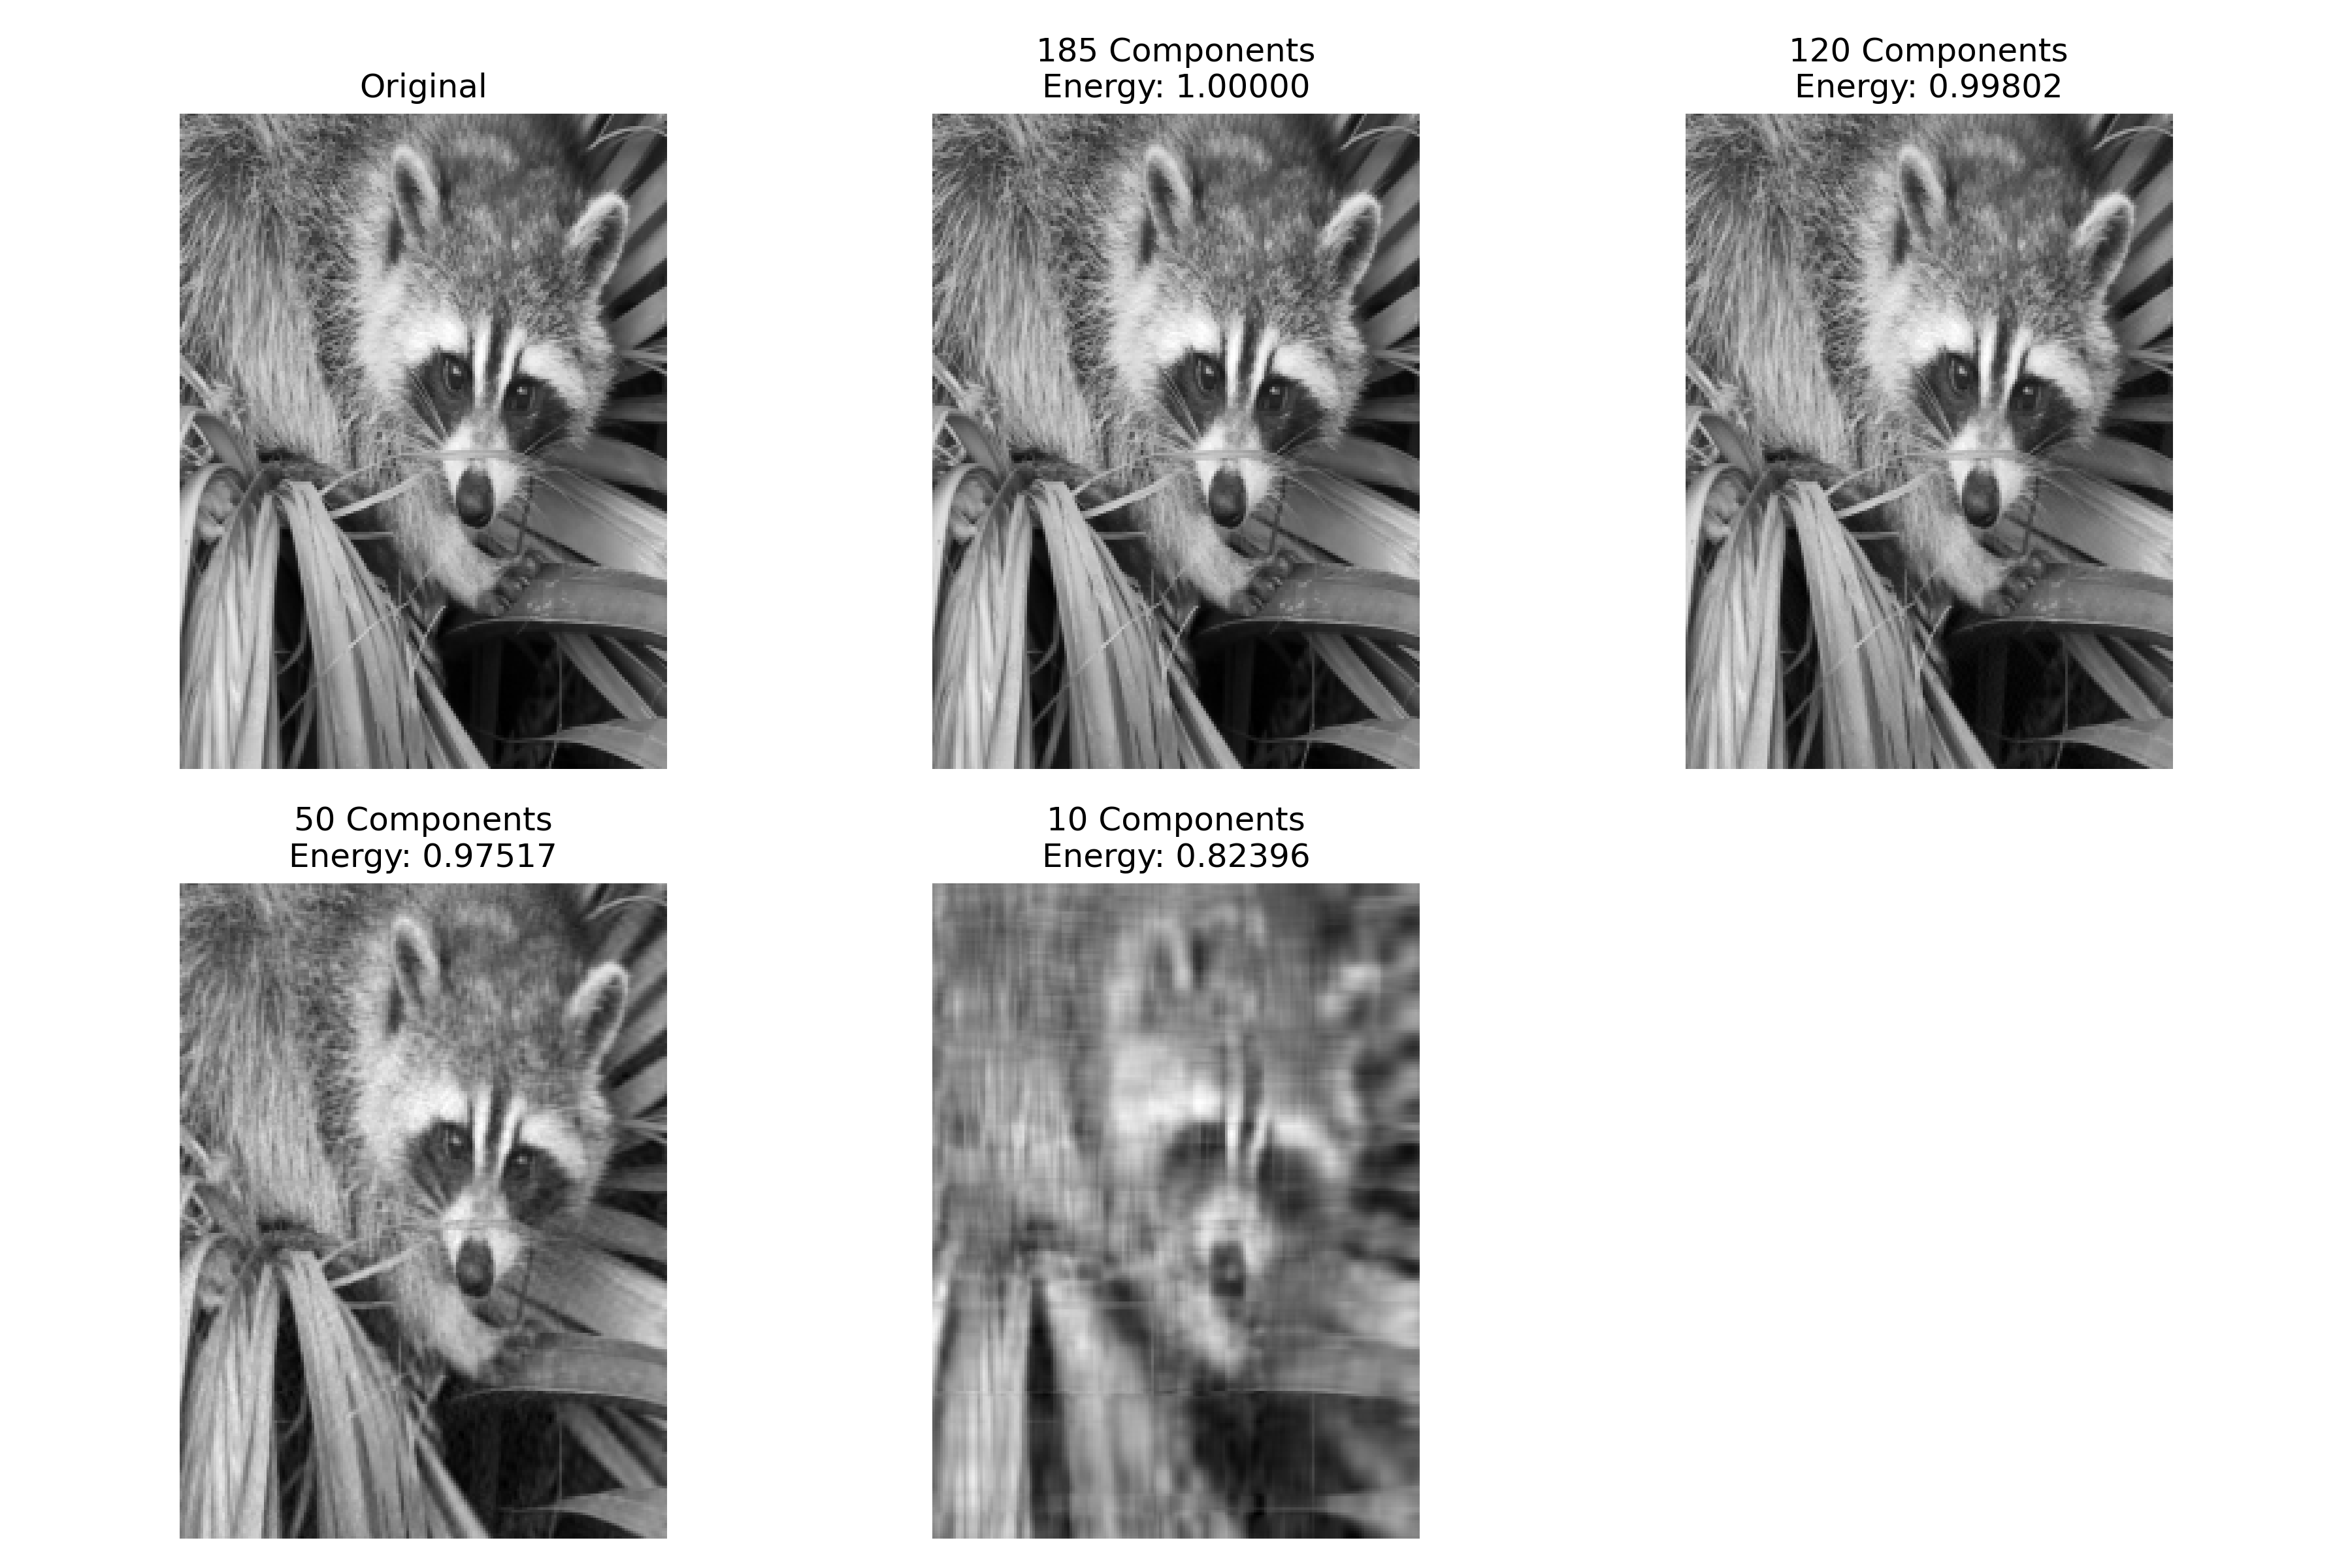
\includegraphics[width=\textwidth]{images/ex3task1-2-2.png}
        \caption{Image Reconstruction Using PCA}
        \label{fig:pca_reconstruction}
    \end{subfigure}
    \caption{PCA on Image Data}
    \label{fig:part2}
\end{figure}

The image dimensions are adjusted to a width of 249 pixels (x-axis) and a height of 185 pixels (y-axis), aligning with the conventional Cartesian coordinate system where 'x' represents the horizontal axis (number of columns) and 'y' represents the vertical axis (number of rows). We then apply Principal Component Analysis (PCA) to this resized image and reconstruct it using varying numbers of principal components. This process allows us to examine the impact of different component counts on the quality of the reconstructed image.


In Figure \ref{fig:part2}, the original image is displayed alongside its PCA reconstructions with varying numbers of components. As the number of components decreases, the clarity of the reconstruction correspondingly diminishes. Retaining all 185 components, which match the image's column count, maintains most of the image's variance. Analysis of the variance captured by different numbers of components reveals that 120 components account for 99.802\% of the variance, 50 components for 97.517\%, and 10 components for 82.396\%.

% P2: At what number is the information loss visible?
Information loss becomes visibly evident when the number of components falls well below the total column count of 185. Particularly, with 50 components, where 97.517\% of the variance is explained, the degradation in detail and sharpness starts to be perceptible.

% P2: At what number is the energy lost through truncation smaller than 1\%?
The truncation's energy loss is less than 1\% when 120 components are used since they explain 99.802\% of the variance, indicating a minimal remainder of energy loss.

What we learned from the results of PCA.
    \begin{itemize} 
    \item This illustrates the inherent compromise in PCA, there's a balance between the accuracy of the reconstructed data and the number of principal components used. A reduction in components leads to a more abstract and less detailed reconstruction, trading precision for reduced dimensionality. Comparing reconstructions with varying numbers of PCs can aid in grasping the data's complexity and in determining the necessary number of PCs to capture the image(data)'s essential patterns.
    \end{itemize}



% \begin{figure}[H]\ContinuedFloat
%     \centering
%     \begin{subfigure}[b]{0.7\textwidth}
%         \centering
%         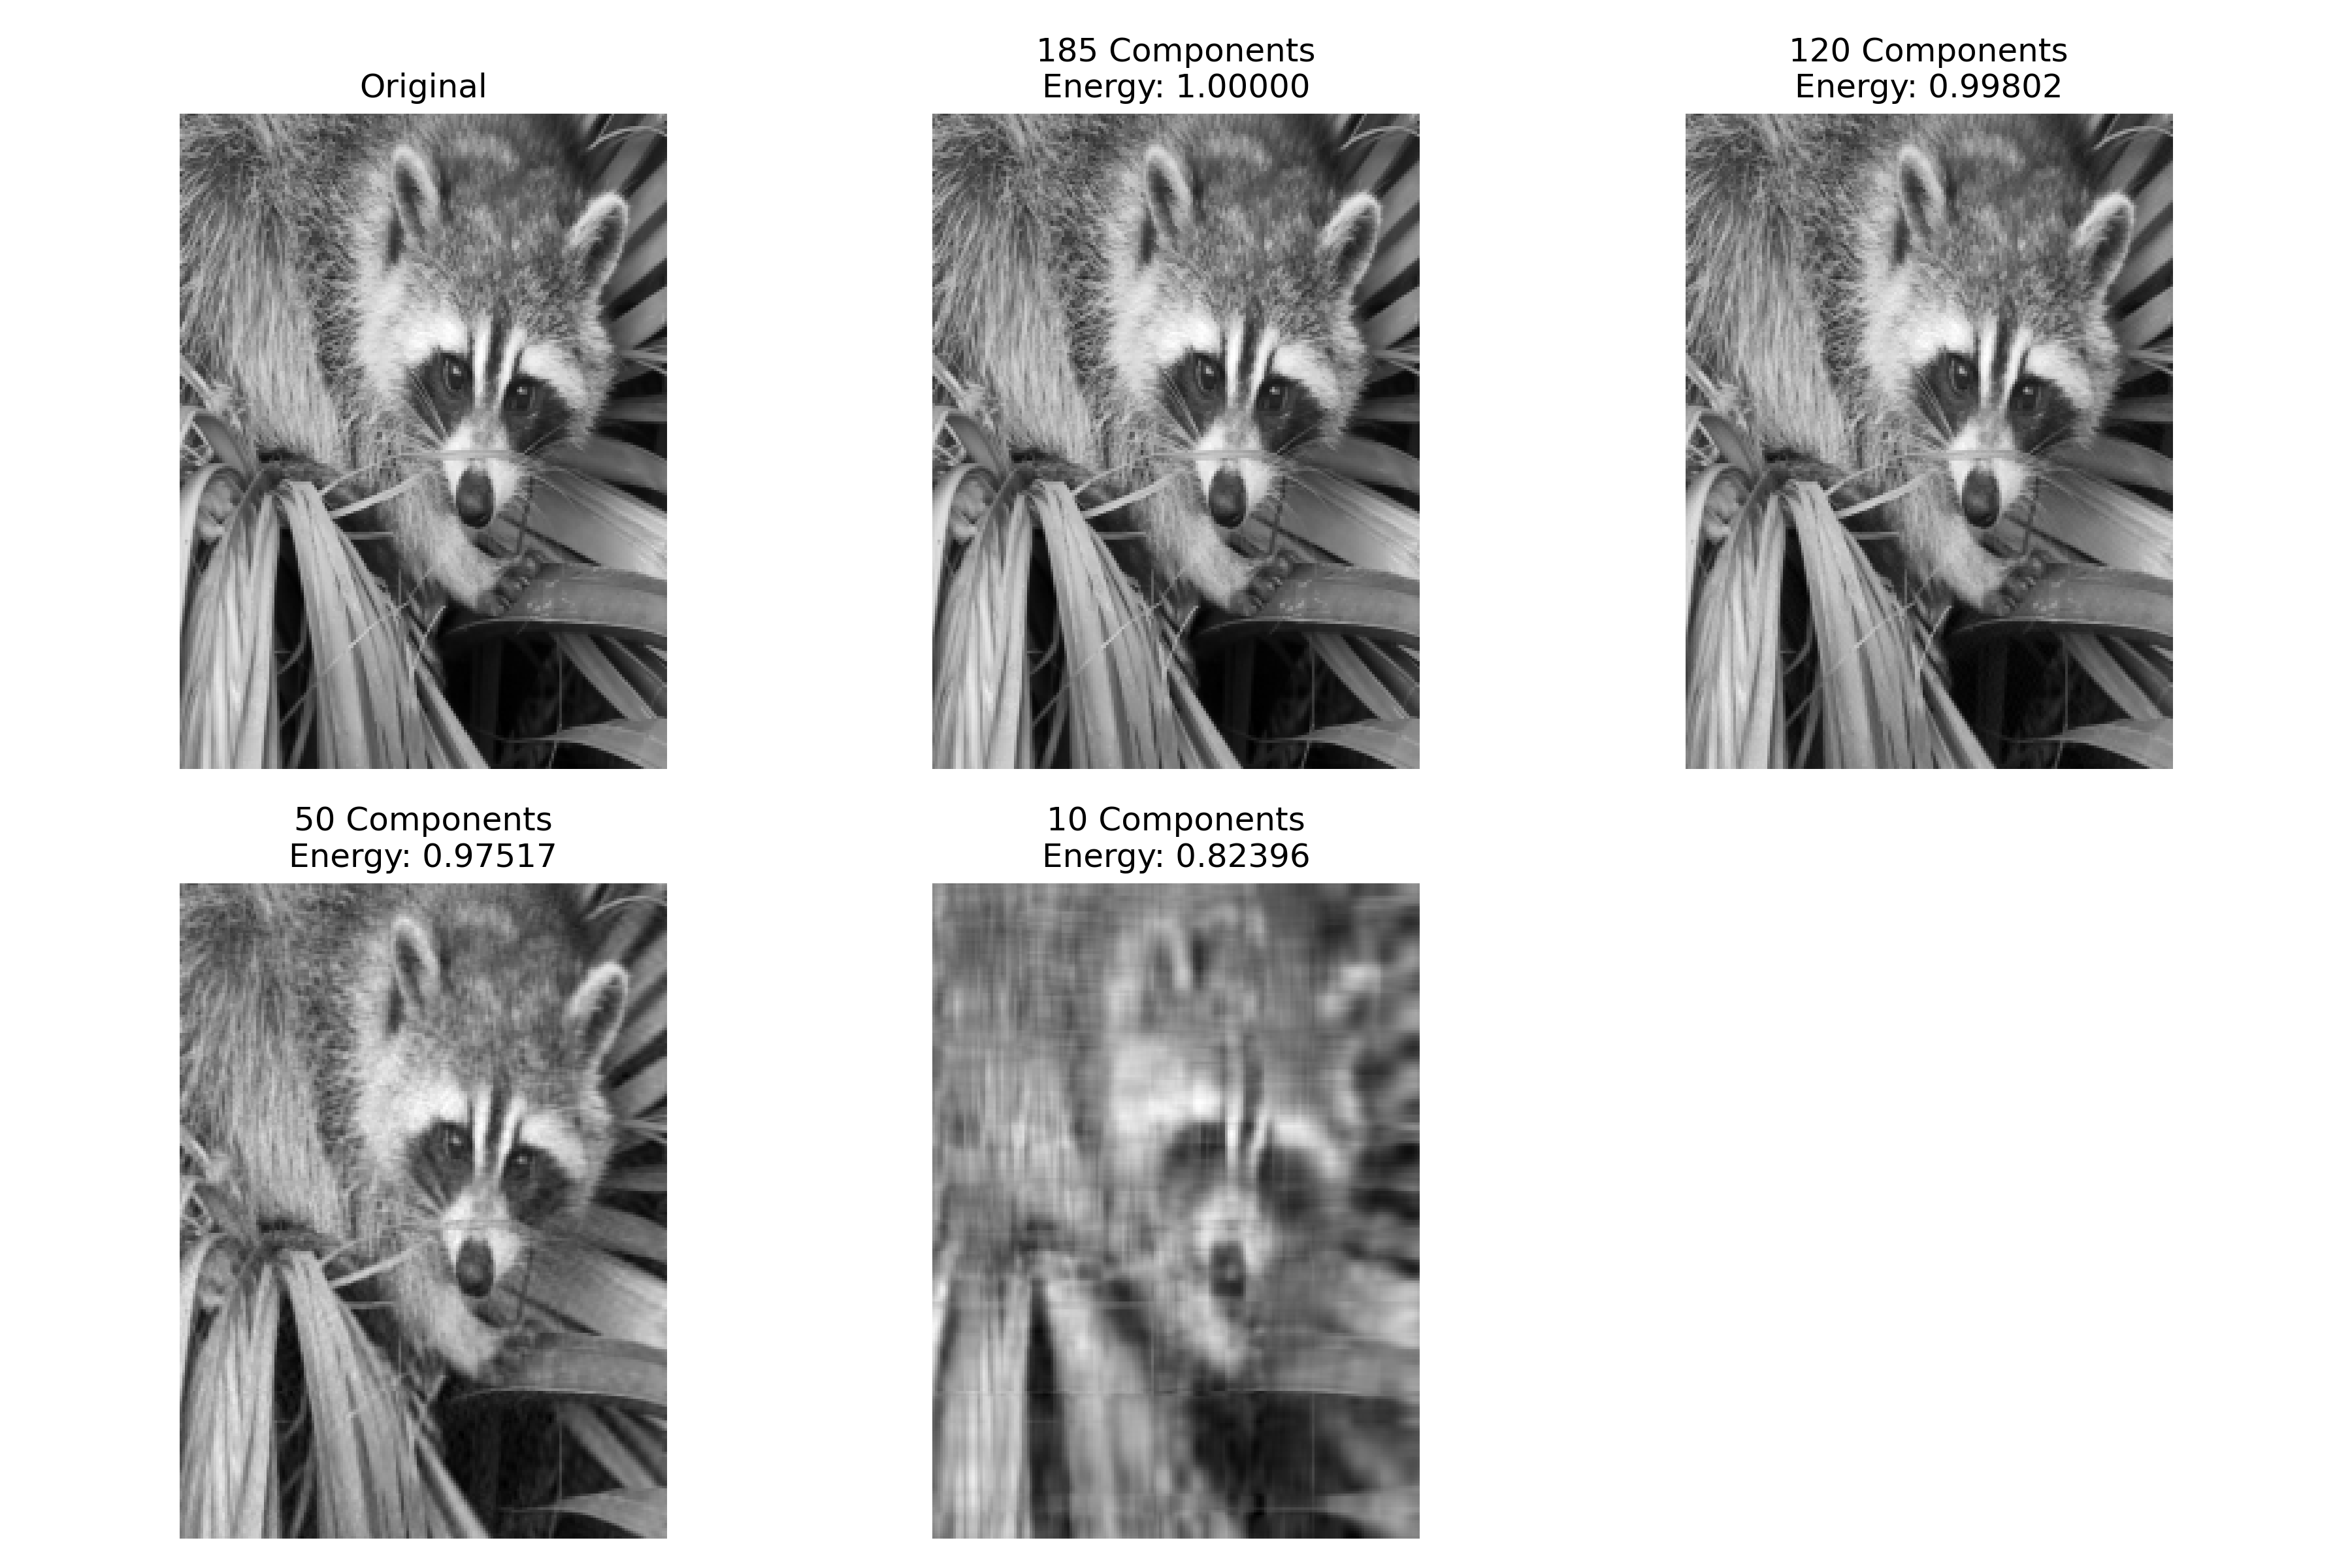
\includegraphics[width=\textwidth]{images/ex3task1-2-2.png}
%         \caption{Image Reconstruction Using PCA}
%         \label{fig:pca_reconstruction}
%     \end{subfigure}
%     \caption{PCA on Image Data}
%     \label{fig:part22}
% \end{figure}





\item \textbf{Part 3:} \\
Part 3 involves analyzing the trajectory data of 15 people. We specifically focus on visualizing the paths of the first two pedestrians in a 2D space.

\begin{figure}[H]
    \centering
    \begin{subfigure}[b]{0.8\textwidth}
        \centering
        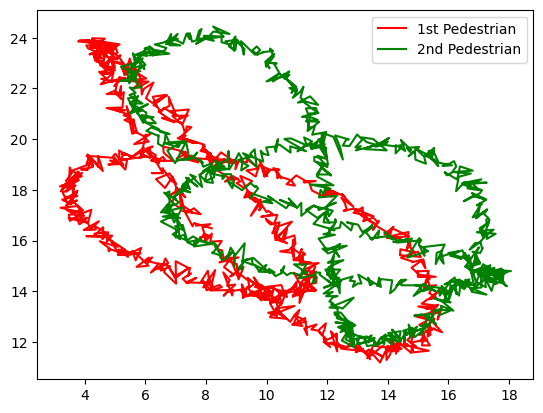
\includegraphics[width=\textwidth]{images/ex3task1-3-1.png}
        
        \label{fig:original_trajectory_pedestrians}
    \end{subfigure}
    \caption{Original Trajectory of Pedestrian 1,2}
    \label{fig:part3-1}
\end{figure}


The trajectories in figure \ref{fig:part3-1} exhibit circular movement patterns and show the raw tracking data, which is replete with noise and jagged lines, capturing all the variance but lacking the detail needed to fully describe the complexity of the pedestrians' paths.

\begin{figure}[H]
    \centering
    \begin{subfigure}[b]{0.45\textwidth}
        \centering
        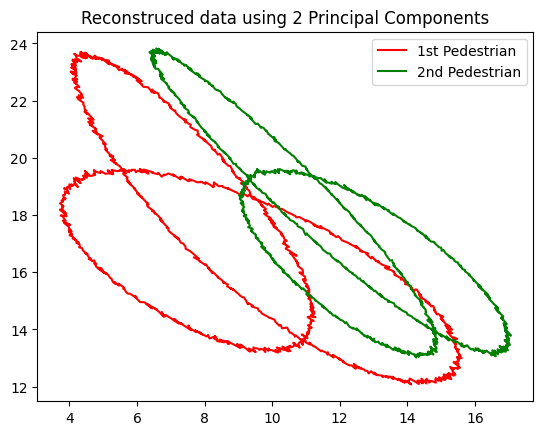
\includegraphics[width=\textwidth]{images/ex3task1-3-2.png}
        \caption{Trajectory of Pedestrian 1,2 with 2 components}
        \label{fig:Trajectory of Pedestrian 1,2 with 2 component3}
    \end{subfigure}
    \begin{subfigure}[b]{0.45\textwidth}
        \centering
        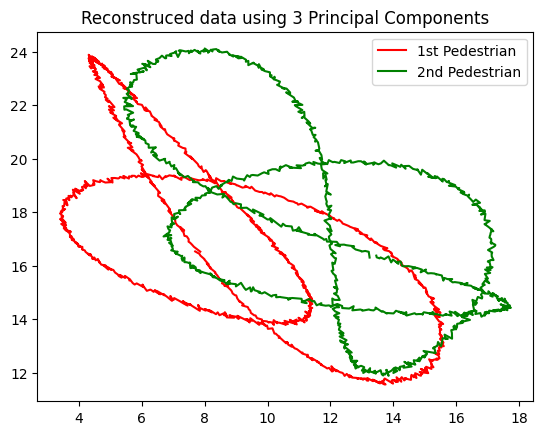
\includegraphics[width=\textwidth]{images/ex3task1-3-3.png}
        \caption{Trajectory of Pedestrian 1,2 with 3 component}
        \label{fig:Trajectory of Pedestrian 1,2 with 3 component}
    \end{subfigure}
    \caption{PCA on Pedestrian Trajectories}
    \label{fig:part3-2}
\end{figure}

In figure \ref{fig:Trajectory of Pedestrian 1,2 with 2 component3}, PCA with 2 components is shown. The trajectories are still distinguishable but have lost some detail compared to the multi-component reconstruction. The paths are broader and less precise, indicating that the third principal component may have contained information that contributed to a more nuanced description of the motion. The variance explained by each component is [0.47320404, 0.37601352], with an overall explained variance of approximately 0.849. Given the complex nature of the trajectories, two components are insufficient to capture the majority of the dataset's energy. The explained variance with 2 components is below 90\%.

Consequently, we are considering using more than 2 components, specifically 3 components, as depicted in figure \ref{fig:Trajectory of Pedestrian 1,2 with 3 component}. The circular patterns in the data introduce complexity that requires additional dimensions for an accurate representation. To capture more than 90\% of the variance, at least 3 components are necessary, As a result, the 3-component plot shows a fairly smooth and well-defined trajectory for both pedestrians. The use of three principal components suggests that this is a higher-fidelity reconstruction of their movement, retaining more detail of the motion paths. This is also evidenced by the increase in explained variance to approximately 0.997 with 3 components. the variance explained is [0.47320404, 0.37601352, 0.14791464], resulting in an overall explained variance of approximately 0.997.

What we learned from the results of PCA.

\begin{itemize}
    \item PCA is used to reduce the dimensionality of data, which could be very high-dimensional if it includes many tracked points or is sampled at a high frequency. This leads to noise filtering, as higher-order components may correspond to less significant movements or noise. By utilizing fewer principal components, the data can be compressed, retaining the most critical information which might suffice for some applications such as basic movement analysis or pattern recognition.
    \end{itemize}

\end{itemize}


% time estimate 
The development and implementation of the PCA code took approximately 2 hours, with a significant portion of this time dedicated to the intricacies of PCA itself. The volumne of data itself was relatively small, so implementing it did not take significant time. 

%Accuracy Considerations 
Accuracy for model is commonly evaluated using metrics such as Mean Squared Error (MSE). However, the nature of our datasets doesn't comply with model accuracy. For the first dataset, which is two-dimensional, employing PCA does not reduce dimensionality but rather linearizes the data. Given its limited variable count, conventional model evaluation techniques are not applicable. The second dataset, being an image, and the third dataset, consisting of pedestrian's trajectory data, also have characteristics that limit the suitability of standard modeling approaches. 

Therefore, we have opted to consider the 'energy' retained in the principal components as an alternative measure of accuracy for these datasets. It's essential to understand that while this method offers insight into the variance captured by PCA, it does not provide a comprehensive assessment of model accuracy in the same manner as error metrics like MSE. Moreover, it is important to recognize that applying PCA does not necessarily improve MSE or other error metrics, as the effectiveness of PCA largely depends on the specific characteristics and requirements of the data being analyzed.

% what we learned
% We learned about PCA.
% Data. 

% Verbose discussion of the results in the report?
% Code: modular, concise, well documented?

